\documentclass[12pt,a4paper]{article}
\usepackage[utf8]{inputenc}
\usepackage[english]{babel}
\usepackage{enumerate}
\usepackage{amsmath}
\usepackage{amsfonts}
\usepackage{amssymb}
\usepackage{graphicx}
\usepackage{fourier}
\usepackage[left=2cm,right=2cm,top=2cm,bottom=2cm]{geometry}
\usepackage{commath}
\usepackage{cancel}
\usepackage{placeins}

\author{Juan Carlos Apitz, ID 012523821}
\title{STAT572 - Final Assignment}
\begin{document}

\maketitle
\nocite{*}

\clearpage

\section*{Question 1}

\subsection*{Part a}
In this problem the model is specified as follows:
\[X|\delta\sim f(x|\delta)=\delta N(\mu_1,\sigma_1^2)+(1-\delta)N(\mu_2,\sigma_2^2)\]
\[\delta\sim h(\delta)=\text{Unif}(0,1)\]
And the likelihood used to build the chain is:
\[L(X_i) = \Pi_{i=1}^n\Bigr[\delta N(\mu_1,\sigma_1^2)+(1-\delta)N(\mu_2,\sigma_2^2)\Bigr]\]

The estimates of the mean and variance, $90\%$ confidence interval and mix rate are given below.
\begin{verbatim}
The Monte Carlo Estimate of the mean is 0.794265

The Monte Carlo Estimate of the variance is 0.000865

The 90 percent Confidence Interval is: (0.792735, 0.795795)

The mix rate is 9.64 percent.
\end{verbatim}

Notice that this particular model yields a mix rate that is too low at $9.6\%$. And in figure \ref{q1fig1} below we see graphically that the chain has poor mixing getting "stuck" in various states.  

\begin{figure}[ht!] 
\begin{center}
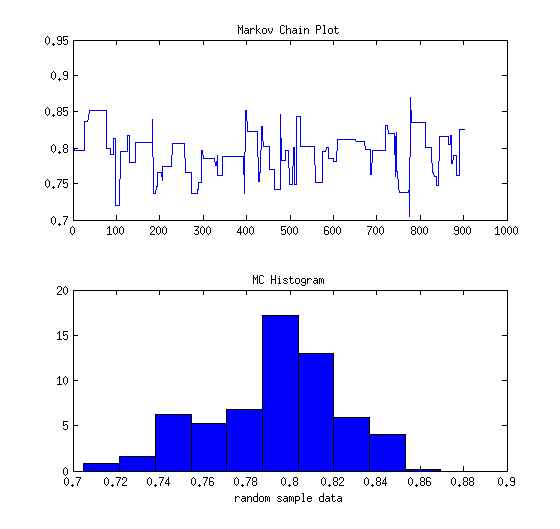
\includegraphics[scale=.7]{q1graph1.png}
\caption{This models shows a poor mixing rate.}
\label{q1fig1}
\end{center}
\end{figure}
\FloatBarrier
\clearpage
\textbf{Code for Question 1.a}\\
\begin{verbatim}

addpath ~/Documents/Stat572/CompStatsToolboxV2
load('Finalpr1.mat')
%%
% ESTIMATE PARAMETERS WITH EM ALGO
% initialize parameters
muin = [2 5]; piesin = [0.5 0.5]; varin = [1 1]; data = y;
max_it = 100; tol = 0.001;
% run EM
[pies,mus,vars]=csfinmix(data,muin,varin,piesin,max_it,tol);
% set up the likelihood function
% likelihood = @(x,mu1,mu2,sigma1,sigma2,delta)...
%     exp(sum(log(delta*normpdf(x,mu1,sqrt(sigma1))+...
%     (1-delta)*normpdf(x,mu2,sqrt(sigma2)))));
likelihood = @(x,mu1,mu2,sigma1,sigma2,delta) prod(delta*normpdf(x,mu1,sqrt(sigma1))+...
    (1-delta)*normpdf(x,mu2,sqrt(sigma2)));
%%
% GENERATE THE MC
% Generate n samples in the chain.
n = 1000; % random sample size
burn = 0.1*n; % burn-in rate
M = 100; % set up Monte Carlo iterations
MCmu = zeros(M,1); MCvar = zeros(M,1);
mixrate = zeros(M,1); % count the mix rate
for j = 1:M
    % initialize the chain
    mc = zeros(1,n);
    mc(1) = rand(1); % generate the starting point
    mixcount = 0; % count the mix rate
    for i = 2:n
        % generate a candidate from the chosen prior
        x = unifrnd(0,1);
        % generate a uniform for comparison
        u = rand(1);
        alphaf = min([1, likelihood(data,mus(1),mus(2),vars(1),vars(2),x)/...
            (likelihood(data,mus(1),mus(2),vars(1),vars(2),mc(i-1)))]);
        if u <= alphaf
            mc(i) = x;
            mixcount = mixcount+1;
        else
            mc(i) = mc(i-1);
        end
    end
    MCmu(j) = mean(mc(burn:n)); MCvar(j) = var(mc(burn:n));
    mixrate(j) = mixcount/n;
end
%%
% PROVIDE HISTOGRAM
figure(1)
subplot(211)
plot(mc(burn:n))
title('Markov Chain Plot')
[fhath, bc] = hist(mc(burn:n));
fhath = fhath/((bc(2)-bc(1))*sum(fhath));
subplot(212)
bar(bc,fhath,1,'b')
title('MC Histogram')
xlabel('random sample data')

% MIX RATE
mixrate = mean(mixrate);

% PROVIDE MC ESTIMATE OF MEAN AND VARIANCE
MCxbar = mean(MCmu); MCssq = mean(MCvar);

% CONSTRUCT 90% CI FOR MEAN OF DELTA
% Get the value for z_alpha/2
alpha = 0.1;
zlo = norminv(1-alpha/2,0,1);
zhi = norminv(alpha/2,0,1);
thetalo = MCxbar - zlo*sqrt(MCssq/n);
thetaup = MCxbar - zhi*sqrt(MCssq/n);
fprintf('\nThe Monte Carlo Estimate of the mean is %2.6f\n', MCxbar)
fprintf('\nThe Monte Carlo Estimate of the variance is %2.6f\n', MCssq)
fprintf('\nThe 90 percent Confidence Interval is: (%2.6f, %2.6f)\n',thetalo, thetaup)
fprintf('\nThe mix rate is %2.2f percent.\n', mixrate*100)

\end{verbatim}

\subsection*{Part b}
In this problem the model is specified as follows:
\[X|\delta\sim f(x|\delta)=\delta N(\mu_1,\sigma_1^2)+(1-\delta)N(\mu_2,\sigma_2^2)\]
\[\delta\sim h(\delta)=\text{Beta}(80.8,15.0)\]
The estimates of the mean and variance, $90\%$ confidence interval and mix rate are given below.
\begin{verbatim}
The Monte Carlo Estimate of the mean is 0.835477

The Monte Carlo Estimate of the variance is 0.000121

The 90 percent Confidence Interval is: (0.834905, 0.836049)

The mix rate is 63.65 percent.
\end{verbatim}
Notice that this particular model yields a much better mix rate now at $63.7\%$. And in figure \ref{q1fig2} below we see graphically that the chain converges to its stationary state much more quickly. 

\begin{figure}[ht!] 
\begin{center}
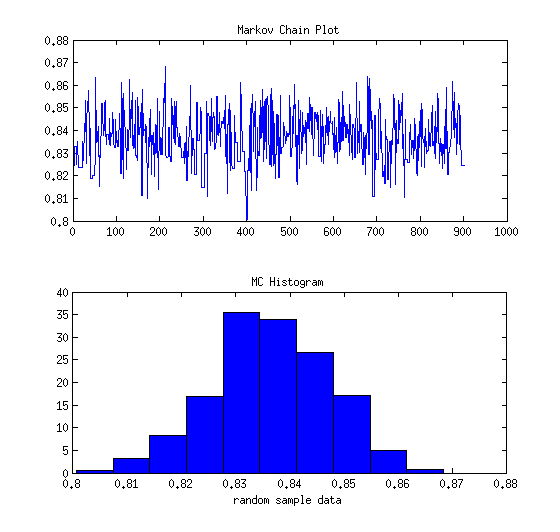
\includegraphics[scale=.7]{q1graph2.png}
\caption{With this model and choice of parameters for the proposal, the mixing rate is improved.}
\label{q1fig2}
\end{center}
\end{figure}
\FloatBarrier

\textbf{Explanation of the Choice of the Beta Parameters}\\
The mixing rate at which a proposal observation is accepted depends to a great extent on our choice of proposal distribution. According to Roberts \cite{roberts2004general} a proposal whose variance is too large relative to the the empirical distribution will generally produce poor mixing rates. Thus to choose the parameters for the proposal in this exercise, we used a variance estimate based on the MC produced in part a) and then solved numerically for the roots of:
\[\dfrac{\alpha\beta}{(\alpha+\beta)^2(\alpha+\beta+1)}-	8.65\times 10^{-5}=0\]
This produced values for $\beta$ and $\alpha$ that were very large and when used in the model produced mixing rates of over $90\%$. A high mixing rate is also not desirable see Roberts \cite{roberts1997weak}. However, we can scale this variance or parameters to produce acceptable mixing rates. The scaled values we chose were $\alpha=80.8$ and $\beta=15.0$. Using these parameter values we were able to obtain a mixing rate of 63.65\%.
\clearpage

\textbf{Code for Question 1.b}\\
\begin{verbatim}

addpath ~/Documents/Stat572/CompStatsToolboxV2
load('Finalpr1.mat')
%%
% ESTIMATE PARAMETERS WITH EM ALGO
% initialize parameters
muin = [2 5]; piesin = [0.5 0.5]; varin = [1 1]; data = y;
max_it = 100; tol = 0.001;
% run EM
[pies,mus,vars]=csfinmix(data,muin,varin,piesin,max_it,tol);
% set up likelihood function
likelihood = @(x,mu1,mu2,sigma1,sigma2,delta)...
    exp(sum(log(delta*normpdf(x,mu1,sqrt(sigma1))+...
    (1-delta)*normpdf(x,mu2,sqrt(sigma2)))));
%%
% GENERATE THE MC
% Generate n samples in the chain.
n = 1000; % random sample size
burn = 0.1*n; % burn-in rate
M = 100; % set up Monte Carlo iterations
MCmu = zeros(M,1); MCvar = zeros(M,1);
mixrate = zeros(M,1); % count the mix rate
% OPTIMIZER
BETAVAR = @(theta) theta(1)*theta(2)/((theta(1) + theta(2))^2*(theta(1)+...
    theta(2)+1))-0.000865;
theta = fminsearch(BETAVAR,[1, 1]); scale = 10^16;
for j = 1:M
    % initialize the chain
    mc = zeros(1,n);
    mc(1) = rand(1); % generate the starting point
    mixcount = 0; % count the mix rate
    for i = 2:n
        % generate a candidate from the chosen prior
        x = betarnd(theta(1)/scale,theta(2)/scale);
        % generate a uniform for comparison
        u = rand(1);
        alphaf = min([1, likelihood(data,mus(1),mus(2),vars(1),vars(2),x)/...
            (likelihood(data,mus(1),mus(2),vars(1),vars(2),mc(i-1)))]);
        if u <= alphaf
            mc(i) = x;
            mixcount = mixcount+1;
        else
            mc(i) = mc(i-1);
        end
    end
    MCmu(j) = mean(mc(burn:n)); MCvar(j) = var(mc(burn:n));
    mixrate(j) = mixcount/n;
end
%%
% PROVIDE HISTOGRAM
figure(1)
subplot(211)
plot(mc(burn:n))
title('Markov Chain Plot')
[fhath, bc] = hist(mc(burn:n));
fhath = fhath/((bc(2)-bc(1))*sum(fhath));
subplot(212)
bar(bc,fhath,1,'b')
title('MC Histogram')
xlabel('random sample data')

% MIX RATE
mixrate = mean(mixrate);

% PROVIDE MC ESTIMATE OF MEAN AND VARIANCE
MCxbar = mean(MCmu); MCssq = mean(MCvar);

% CONSTRUCT 90% CI FOR MEAN OF DELTA
% Get the value for z_alpha/2
alpha = 0.1;
zlo = norminv(1-alpha/2,0,1);
zhi = norminv(alpha/2,0,1);
thetalo = MCxbar - zlo*sqrt(MCssq/n);
thetaup = MCxbar - zhi*sqrt(MCssq/n);
fprintf('\nThe Monte Carlo Estimate of the mean is %2.6f\n', MCxbar)
fprintf('\nThe Monte Carlo Estimate of the variance is %2.6f\n', MCssq)
fprintf('\nThe 90 percent Confidence Interval is: (%2.6f, %2.6f)\n',thetalo, thetaup)
fprintf('\nThe mix rate is %2.2f percent.\n', mixrate*100)

\end{verbatim}
\clearpage

\section*{Question 2}
\textbf{Procedure}\\
For this problem we generate a random sample from Poisson$(\lambda=1)$ by implementing the following steps:
\begin{enumerate}
\item{First we generate j random variables Y$\sim Exp(\lambda=1)$;}
\item{Then generate 100 random variables X by calculating $X_i=\sum_{j=1}^iY_j$, with $i = 1, 2, ..., 100$;}
\item{Next we calculate $Z = \#\{X_i : X_i \in [l-1,l\}$, where $l\geq1$.}
\end{enumerate}
The table below shows the frequency count by category of the random variable $Z$ for $l = 2,4,8,16$. It seems that the choice of the parameter $l$ does not change the frequency distribution of $Z$.

\begin{verbatim}
               Count_2    Count_4    Count_8    Count_16
               _______    _______    _______    ________

    0 to 1     411        409        401        397     
    1 to 2     208        198        182        199     
    2 to 3      42         54         62         55     
    3 to 4       5          9          8         14     
    4 to 5       0          1          1          5    

\end{verbatim}

\textbf{Comparison to Theoretical Poisson}\\
Figure \ref{q2fig1} below shows on the left graph a histogram of the random sample generated by the process outlined above. The graph on the right shows the theoretical distribution of a Poisson random variable with $\lambda=1$. The distribution of our random sample, as expected, resembles the theoretical distribution.

\begin{figure}[ht!] 
\begin{center}
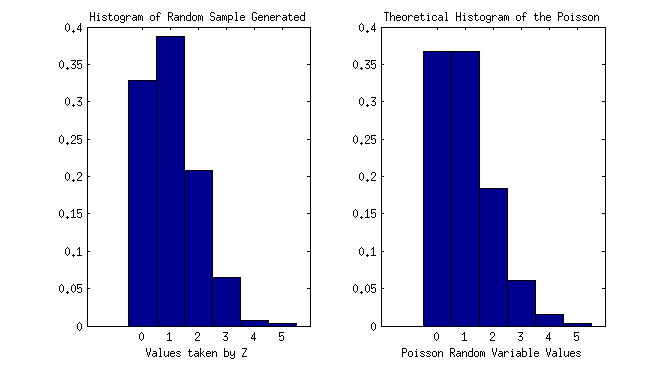
\includegraphics[scale=.9]{q2graph1.png}
\caption{Poisson Random Sample vs. Theoretical Distribution.}
\label{q2fig1}
\end{center}
\end{figure}
\FloatBarrier
\clearpage
\textbf{Code}\\
\begin{verbatim}
function [Z] = poissonRandom(lam,l,k,n)
%%%%%%%%%%%%%%%%%%%%%%%%%%%%%%%%%%%%%%%%%%%%%%%%%%%%%%%%%%%%%%%%%%%%%%%%%
% inputs: lam = parameter for the poisson; l = parameter for Z interval %
%         k = size of X, n = size on random sample                      %
%%%%%%%%%%%%%%%%%%%%%%%%%%%%%%%%%%%%%%%%%%%%%%%%%%%%%%%%%%%%%%%%%%%%%%%%%
% GENERATE Xi
% initialize
X = zeros(k,1);
Z = zeros(n,1);
for j = 1:n
    for i = 1:k
        % Generate the exponential random variables.
        uni = rand(1,i);
        y = -log(uni)/lam;
        X(i) = sum(y);
    end
    hits = X >= l-1 & X<l;
    Z(j) = sum(hits);
end
edges = 0:max(Z);
fhat = histc(Z,edges);

figure(1)
subplot(121)
bar(edges,fhat/n,1)
subplot(122)
bar(0:5,poisspdf(0:5,1),1)
\end{verbatim}
\clearpage
\subsubsection*{Part a}
In this part of the exercise we use the Bootstrap resampling method to generate a 1000 Poisson random samples and estimate the distribution of these samples:
\begin{enumerate}
\item{First we generate a Poisson random sample of size 100 with $\lambda=1$ using the Poisson/Exponential relationship as outlined above.}
\item{Then we take 2000 random samples without replacement from the original size 100 Poisson sample. This generates a 100 by 200 matrix of observations.}
\item{For each of the columns of the matrix above (these are the Bootstrap samples) we calculate the frequency for categories 0 to 1, 1 to 2,..., 9 to 10, 10+.}
\item{Finally, we take the mean of each frequency category which is an estimate of probability mass function $\hat{p}(x)$.}
\end{enumerate}
Figure \ref{q2fig2} below shows the comparison of this probability mass function with the distribution of a theoretical Poisson distribution with $\lambda=1$. Clearly, our estimate closely resembles the theoretical distribution.

\begin{figure}[ht!] 
\begin{center}
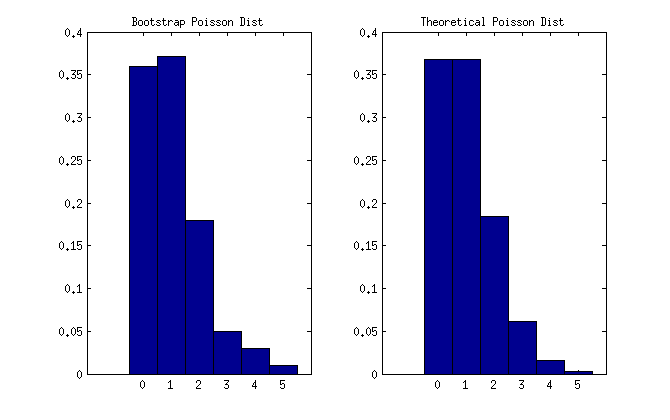
\includegraphics[scale=.9]{q2graph2.png}
\caption{Bootstrap Density Estimate vs. Theoretical Poisson Density.}
\label{q2fig2}
\end{center}
\end{figure}
\FloatBarrier

A numerical comparison also shows close fit:
\begin{verbatim}
Theoretical Poisson =

    0.3679    0.3679    0.1839    0.0613    0.0153    0.0031
    
Estimated with Bootstrap =

    0.3703    0.3604    0.1790    0.0707    0.0196
\end{verbatim}
\clearpage
\textbf{Code}
\begin{verbatim}
% generate sample data from exponential of size k
lam = 1; k = 100; l = 5;
SampleY = zeros(k,k);
Z = zeros(1,k);
for j = 1:k
    for i = 1:k
        SampleY(i,1:i) = exprnd(lam,1,i);
    end
    SampleX = sum(SampleY,2);
    hits = SampleX >= l-1 & SampleX<l;
    Z(j) = sum(hits);
end

% generate B bootstraps
B = 2000;
inds = unidrnd(k,k,B);
xboot = Z(inds);
edges = 0:max(Z);
fhat = histc(xboot,edges);
fhat = mean(fhat,2);

figure(1)
subplot(121)
bar(edges,fhat/k,1)
subplot(122)
bar(0:5,poisspdf(0:5,1),1)
\end{verbatim}
\clearpage
\textbf{Part b}\\
In this part we use the method of kernel density estimation to estimate the density of the random sample generated using the Poisson/Exponential relationship:
\begin{enumerate}
\item{First we generate a Poisson random sample of size 1000 with $\lambda=1$ using the methodology that uses the Poisson/Exponential relationship.}
\item{Using this as our data points, we generate a normal kernel centered at each of the 1000 data points with variance $h=1.06s(x)*n^{-\frac{1}{5}}$ and produce a density estimate.}
\end{enumerate}

In figure \ref{q2fig3} below we see the graphical comparison of the two kernel density based on the random sample and the theoretical density of the Poisson distribution with $\lambda=1$. 

\begin{figure}[ht!] 
\begin{center}
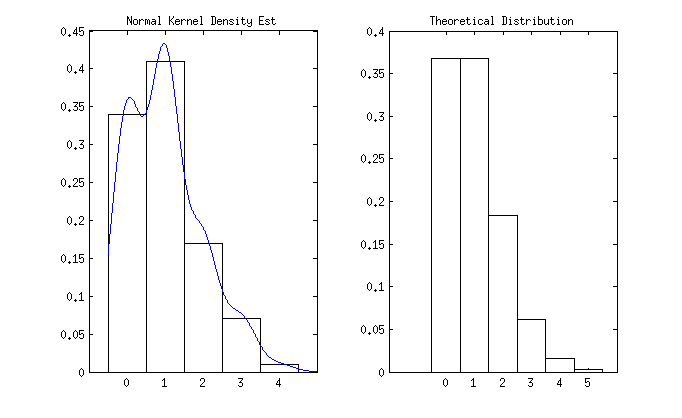
\includegraphics[scale=.9]{q2graph3.png}
\caption{Kernel Density vs. Theoretical Poisson.}
\label{q2fig3}
\end{center}
\end{figure}
\FloatBarrier
\clearpage
\textbf{Code}
\begin{verbatim}
% generate sample data from exponential of size k
lam = 1; n = 1000; l = 5;
SampleY = zeros(n,n);
Z = zeros(1,n);
for j = 1:n
    for i = 1:n
        SampleY(i,1:i) = exprnd(lam,1,i);
    end
    SampleX = sum(SampleY,2);
    hits = SampleX >= l-1 & SampleX<l;
    Z(j) = sum(hits);
end
data = Z;
edges = 0:max(data);
fhat = histc(data,edges);
figure(1)
subplot(121)
bar(edges,fhat/n,1,'w')
hold on

% choose an appropriate domain
x = linspace(-0.5,5,5000); % domain

% choose smoothing parameter
h = 1.06*std(data)*n^(-1/5); 

% evaluate using the normal kernel for each data point 
% at all x in the domain
fhat = zeros(size(x));
for i=1:n
    % get each kernel function evaluated at x
    % centered at data and weighted by h
    f=exp(-(1/(2*h^2))*(x-data(i)).^2)/sqrt(2*pi)/h;
    % add each ith average f vector to get estimate pdf height
    fhat = fhat+f/(n);
end
linenorm = plot(x,fhat,'b');

hold off
subplot(122)
bar(0:5,poisspdf(0:5,1),1,'w')

\end{verbatim}
\clearpage

\section*{Question 3}
\textbf{Starting Values: $\mathbf{x_0=y_0=20}$.}\\
When we use an over dispersed starting value for both variables such as 20, we see that without a burn-in period the chain has to converge from the starting point of $x_0=y_0=20$ to a stationary process where the chain is constrained to the interval $0<x_i<10$. (see figure \ref{q3fig1} below). We see that the measures of centrality (the mean) and dispersion (the variance) are not as affected as the the coefficients of skewness and kurtosis (see MATLAB results below). This makes sense because the shape of the distribution is more affected by over dispersed values and with $n=1000$ the mean and variance are not as affected by the choice of initial values.
\begin{verbatim}

                     Mean     Variance    Skewness    Kurtosis
                    ______    ________    ________    ________

    Pre Burn-in     2.3749    7.0736      1.4895       5.275  
    Post Burn-in    2.3101    6.6958       1.348      3.8369  
\end{verbatim}

The marginal pdf point estimates for $x=0.1, 1.8, 3.5, 9.2$ are:
\begin{verbatim}
fhat =

    1.5579    0.0781    0.0303    0.0053
\end{verbatim}

\begin{figure}[ht!] 
\begin{center}
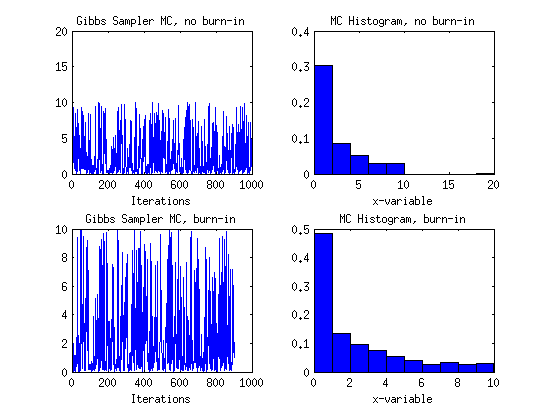
\includegraphics[scale=1]{q3graph1.png}
\caption{caption.}
\label{q3fig1}
\end{center}
\end{figure}
\FloatBarrier
\clearpage

\textbf{Starting Values: $\mathbf{x_0=y_0=2.5}$.}\\
Now using a starting value of 2.5, we see that the chain does not need to converge to a stationary process. In this case, the burn-in period is not as crucial (see figure \ref{q3fig2} below). We also see that the mean, variance, skewness, and kurtosis do not appear significantly different with or without burn-in period (see MATLAB results below). Additionally, the statistics remain more or less consistent between the two MC generated using different starting values. The histograms in figure \ref{q3fig1} and \ref{q3fig2} indicate that the data generated likely comes from an exponential distribution with $\lambda\approx 2.4$.
\begin{verbatim}

                     Mean     Variance    Skewness    Kurtosis
                    ______    ________    ________    ________

    Pre Burn-in     2.3906    6.8389      1.2491      3.5371  
    Post Burn-in    2.4743    6.9895      1.1778      3.3462  
\end{verbatim}
The marginal pdf point estimates for $x=0.1, 1.8, 3.5, 9.2$ are:
\begin{verbatim}
fhat =

    1.4654    0.0869    0.0360    0.0069
\end{verbatim}

\begin{figure}[ht!] 
\begin{center}
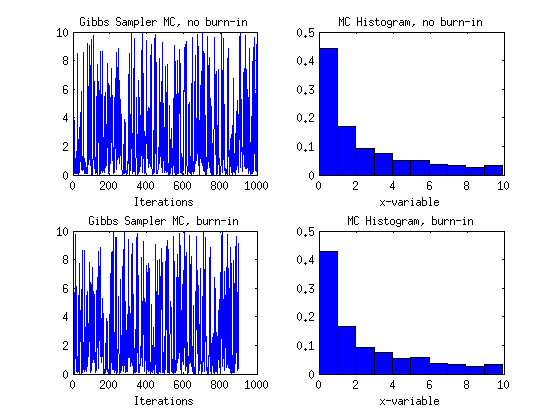
\includegraphics[scale=1]{q3graph2.png}
\caption{caption.}
\label{q3fig2}
\end{center}
\end{figure}
\FloatBarrier
\clearpage

\textbf{Code for Question 3}\\
\begin{verbatim}
%initialize
k = 1000; % generate a chain of size 1000
m = 100; % burn-in
x = zeros(1,k); y = zeros(1,k);
% starting point.
x(1) = 20; %exprnd(1/0.4); 
y(1) = 20; %exprnd(1/x(1));
ind = 2;
while ind < k+1
    xn = exprnd(1/y(ind-1));
    % condition for x domain
    if xn >= 0 && xn <= 10
        x(ind) = xn;
        yn = exprnd(1/x(ind));
        % condition for y domain
        if yn >= 0 && yn <= 10
            y(ind) = yn;
            ind = ind+1;
        end
    end
end

% statistics
Mean = [mean(x); mean(x(m:k))];
Variance = [var(x); var(x(m:k))];
Skewness = [skewness(x); skewness(x(m:k))];
Kurtosis = [kurtosis(x); kurtosis(x(m:k))];
method = {'Pre Burn-in' 'Post Burn-in'};
T = table(Mean, Variance, Skewness, Kurtosis, 'RowNames',method);

% pdf estimate
pdfpt = [0.1 1.8 3.5 9.2];
fhat = zeros(1,length(pdfpt));
for i = 1:length(pdfpt)
    fhat(i) = mean(exppdf(pdfpt(i),y(m:k)));
end

% plots
figure(1)
subplot(221)
plot(x)
title('Gibbs Sampler MC, no burn-in')
xlabel('Iterations')
subplot(222)
[fhath, bc] = hist(x);
fhath = fhath/((bc(2)-bc(1))*sum(fhath));
bar(bc,fhath,1,'b')
title('MC Histogram, no burn-in')
xlabel('x-variable')

subplot(223)
plot(x(m:k))
title('Gibbs Sampler MC, burn-in')
xlabel('Iterations')
subplot(224)
[fhath, bc] = hist(x(m:k));
fhath = fhath/((bc(2)-bc(1))*sum(fhath));
bar(bc,fhath,1,'b')
title('MC Histogram, burn-in')
xlabel('x-variable')
\end{verbatim}
\clearpage

\bibliographystyle{plain}
\bibliography{references}
\end{document}